\section{Network tests and the validity of the closure}
\label{sec:results}

\subsection{Separate recording bias from the dynamical prediction}

The fraction diagnostic was motivated by two 60:40, $N=1000$ realizations
whose original dimension estimates were approximately $0.0135$ and $0.0141$,
against the leading prediction $0.0299$. A pair of unusual networks does
not establish an ensemble bias, and finite-record corrections must be
distinguished from connectivity variation.

The limiting theory predicts infinite-time, neuron-wise centered covariance.
Subtracting a separate empirical mean in each recording block changes that
observable. Appendix~\ref{app:recording} gives an exact mean-difference repair
for independent stationary windows; duration and gap checks test the residual
dependence between windows in actual trajectories.

The existing sixteen-network 60:40 Bernoulli cohort was extended from 4000
to 16000 recorded leak times, preserving each connectivity realization and
initial condition. The original primary-prefix statistics reproduce to
floating-point precision. The standard eight-block estimate changes from
$d=0.027281$ to $0.026041$. At the longer duration, the mean-difference
estimate is $0.025678$ with network standard error $0.001627$ for block
length 500 and a one-block empty gap. Block lengths 1000 and 2000 give
$0.025681$ and $0.025600$ under the corresponding historical gap choice.
The standard-minus-corrected differences decrease approximately as the
inverse block length. This agreement among corrected block choices supports
the estimator repair; it does not prove infinite-time convergence.

The leading parameter-only prediction is $0.029894$, while the retained
formal first-order correction gives $0.030871$ at $N=1000$. Thus the
expanded historical cohort weakens the original factor-two mismatch but
does not establish quantitative agreement. The selected historical seeds
and remaining time and state effects restrict the interpretation of a
network-mean interval. The new prospective comparisons below use fresh
connectivity realizations under a shared estimator protocol.
In this historical cohort, the mean numerator moment is 5.8\% below its
leading value and the mean covariance energy is 9.3\% above. Their
ratio-of-means dimension is approximately $0.02427$, below the mean of
network ratios $0.02568$, as required by Eq.~\eqref{eq:ratiobias}.
This accounting locates the residual in the ingredients; it is not a
parameter-only explanation of why those finite-network shifts occur.

\begin{figure}[t]
\centering
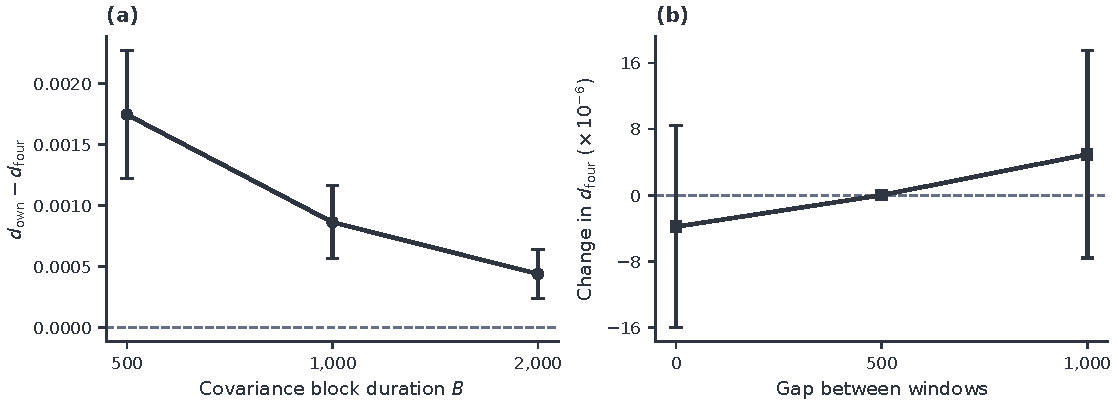
\includegraphics[width=\linewidth]{finite_record_diagnostics.pdf}
\caption{\textbf{Separated windows do not remove their own centering bias.}
Historical sixteen-network Bernoulli 60:40 cohort, $N=1000$, extended to
16000 recorded leak times. (a) The standard separately centered estimate
exceeds the mean-difference estimate at the same block length. Increasing
duration while holding block length fixed does not remove this contribution.
(b) After the repair, changing the minimum empty gap from zero to 1000 leak
times at block length 500 changes mean PR by only a few parts in $10^6$ in
this cohort. Error bars are 95\% Student-$t$ intervals of paired differences
across connectivity realizations; overlapping window quadruples are not
independent network replicates. The panels have different vertical scales.
These checks support this parameter point, not a uniform mixing theorem.}
\label{fig:recording}
\end{figure}

\subsection{The nonuniform degree intervention produces a large dimensionality change}

The degree test uses the nonuniform reference matrices in
Eq.~\eqref{eq:reference}, so that E and I have different local kernels.
The initial eighteen-network allocation contains three fresh connectivity
draws at each of four dispersions for $N=1000$, and three at each endpoint
for $N=2000$. After the quantitative deviations at the larger size, a staged
extension allocated three $N=4000$ networks at each endpoint before observing
those outcomes. All twenty-four networks from this original cohort are retained
in Table~\ref{tab:degree}. Endpoint mean dimensions differ by factors
$7.87$, $7.13$, and $8.41$ at the three sizes, compared with the
parameter-only prediction $10.34$. Thus the large degree effect transfers
to a genuinely nonuniform population profile.

\begin{table}[t]
\centering
\caption{Nonuniform degree test. Measurements are network means with
standard errors. The theoretical value is the ideal requested-dispersion
prediction; integer-count rounding is recorded separately. The initial 18
networks and the staged six-network extension are distinguished in the text.}
\label{tab:degree}
\begin{tabular}{rrrrrr}
\toprule
$N$&$\chi$&$n$&Predicted $d$&Measured $d$&Network SE\\
\midrule
1000&0&3&0.173891&0.149156&0.003542\\
1000&0.5&3&0.055942&0.041364&0.004108\\
1000&1&3&0.034326&0.030165&0.002399\\
1000&2&3&0.016811&0.018960&0.000788\\
2000&0&3&0.173891&0.156176&0.001276\\
2000&2&3&0.016811&0.021896&0.000997\\
4000&0&3&0.173891&0.162277&0.001482\\
4000&2&3&0.016811&0.019306&0.001620\\
\bottomrule
\end{tabular}
\end{table}


In the original cohort, the quantitative discrepancies also transfer. The $N=2000$ endpoint means
are $10.2\%$ below and $30.3\%$ above their respective predictions.
At $N=4000$, these discrepancies are $-6.7\%$ and $+14.8\%$; the
temporal-input-variance errors are about $3.3$--$4.3\%$ across the two
populations and endpoint conditions.
Figure~\ref{fig:degree} displays the local input statistics and absolute
population covariance energies alongside PR. These ingredients show
departures from the limiting law, so the residual cannot be assigned to a
PR ratio alone. Increasing size does not uniformly improve every comparison.
Sensitivity of mean PR to the tested duration and gap choices is only a few
$10^{-4}$ at these degree points: the largest gap shift is $0.000131$ and
the largest 4000-to-8000 duration shift is $0.000461$. Re-solving the conditional equations at
the generator's expected rounded dispersion, while reimposing target means,
changes predicted PR by less than $0.74\%$; this retargeted diagnostic is
kept separate from the primary prediction and is too small to repair the
observed discrepancies.

The follow-up tested twelve dispersions at $N=2000$ with three new networks
at each setting. Three $N=4000$ networks at each of $\chi=0.1,0.75,1.5$
checked selected interior points. In the new $N=2000$ cohort, mean $D/N$
fell from $0.1540$ to $0.0187$ across the endpoints (an 8.24-fold change).
Among the sampled dispersions the largest mean E--E and twice-E--I block
energies occurred at $\chi=0.5$ and $\chi=0.3$, respectively. After four
measurements from the first seed became available, we defined a supplemental
test at the eight dispersions absent from the original sweep. We compared the
root-mean-square error in $\log(D/N)$ for the conditional curve and for the
straight line joining its theoretical endpoints in these coordinates. For
the two independent seeds measured after we chose the test, the errors were
$0.141$ versus $0.455$ and $0.131$ versus $0.428$, respectively. Across all
three seeds, the mean errors were $0.134$ and $0.443$. The descriptive paired
difference was $-0.310$ (95\% interval $[-0.337,-0.282]$).

\begin{figure}[t]
\centering
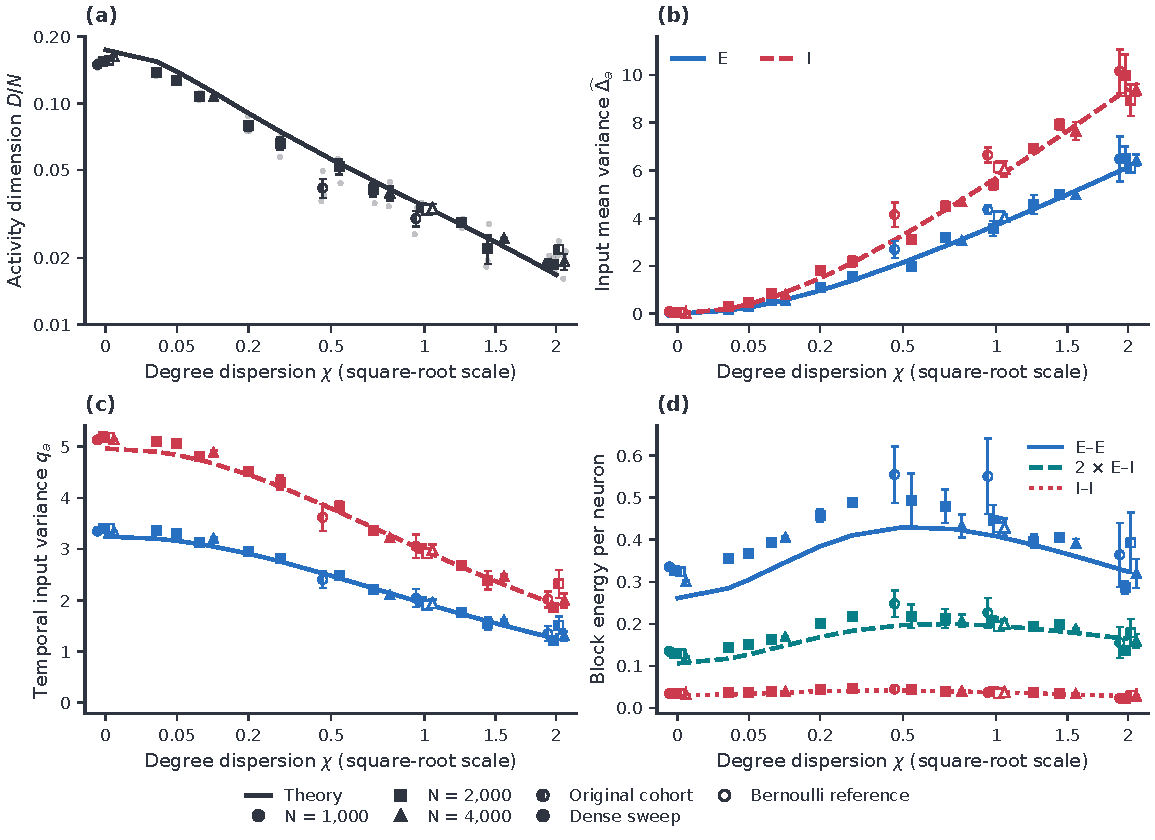
\includegraphics[width=\linewidth]{degree_validation.pdf}
\caption{\textbf{Degree dispersion changes local input statistics and covariance geometry.}
At 80:20 E:I, (a) shows joint dimension per neuron, (b) the across-neuron variance
of finite-record input means, (c) the temporal input variance, and (d) the E--E,
twice E--I, and I--I covariance energies per network neuron. Lines give the
conditional predictions. The square-root scale resolves the closely spaced
dispersions near zero. Marker shape identifies network size. Half-filled symbols
summarize the original 24 networks and filled symbols the 45 new networks.
Each cohort, size, and dispersion has its own mean and one across-network
standard error. Faint dots in (a) are individual realizations. Hollow symbols
at $\chi=1$ give separate Bernoulli references from 12 networks at $N=2000$
and four at $N=4000$. All estimates use 8000 recorded leak times.
The raw input means in (b) retain finite-time sampling noise.}
\label{fig:degree}
\end{figure}

\subsection{Composition and size separate population allocation from absolute accuracy}

The original size series was staged. The initial allocation includes four seed
clusters per composition at $N=1000$ and $N=2000$; after the pilot spread,
the allocation adds eight per composition at $N=2000$ and four per
composition at $N=4000$. Each stage is recorded before its outcomes, every
realization is retained, and first-stage versus additional-seed results are
kept separately. The main observables are $\nu$, $\energy$, $d$, and absolute
population energies. The normalized geometry diagnostics below are
exploratory secondary observables.

In the original $N=2000$ size series, each composition contributed twelve realizations.
The 60:40 means are $\nu=0.151999$, $\energy=0.795195$, and $d=0.029417$,
with relative discrepancies $-0.60\%$, $+1.65\%$, and $-1.59\%$.
The corresponding 80:20 discrepancies are $-1.15\%$, $+2.85\%$, and
$-3.40\%$. For the 60:40 mean dimension, the conventional 95\% relative-error
interval is $[-9.80\%,+6.61\%]$; for 80:20 it is
$[-12.58\%,+5.78\%]$. Across all six moment and dimension means at this
size, interval endpoints range from $-12.58\%$ to $+14.19\%$.
These are descriptive finite-record sampling intervals at the tested
coupling and compositions. They do not bound individual realizations,
establish uniform convergence, or extend the same accuracy to all degree
conditions.
At $N=4000$, the four-network means are $d=0.029973$ at 60:40 and
$d=0.033491$ at 80:20, with relative discrepancies $+0.27\%$ and
$-2.43\%$. Their mean-error intervals are
$[-4.72\%,+5.25\%]$ and $[-17.55\%,+12.68\%]$.
The 60:40 mean numerator and energy are $5.11\%$ and $10.52\%$ above
their leading values; the energy-error interval spans
$[-9.28\%,+30.32\%]$. Thus stable PR does not establish monotone
convergence of the amplitudes or a controlled cancellation of all missing
terms. The more precise $N=2000$ ingredient comparison remains independent
evidence alongside the largest-size PR check.

\begin{table}[t]
\centering
\caption{Fresh composition and size series. Ratios compare the mean of each
network observable with its parameter-only prediction. The interval is a
conventional 95\% Student-$t$ interval for the mean dimension ratio across
independent seed clusters within each condition; it does not include
uncontrolled finite-record bias or provide simultaneous coverage. The
staged allocation and every outcome are retained.}
\label{tab:composition}
\begin{tabular}{rrrrrrr}
\toprule
$f_E$&$N$&$n$&$\bar\nu/\nu_0$&$\bar\energy/\energy_0$&$\bar d/d_0$&95\% interval\\
\midrule
0.6&1000&4&0.869&0.945&0.806&$[0.470,1.142]$\\
0.8&1000&4&0.975&1.100&0.883&$[0.250,1.517]$\\
0.6&2000&12&0.994&1.017&0.984&$[0.902,1.066]$\\
0.8&2000&12&0.988&1.029&0.966&$[0.874,1.058]$\\
0.6&4000&4&1.051&1.105&1.003&$[0.953,1.053]$\\
0.8&4000&4&1.007&1.041&0.976&$[0.825,1.127]$\\
\bottomrule
\end{tabular}
\end{table}


The temporal Gram alignment provides a complementary geometry test.
At $N=2000$, its mean is $0.87217$ at 60:40 and $0.78920$ at 80:20,
against parameter-only values $0.87364$ and $0.79054$. These mean
relative discrepancies are about $0.17\%$, with no fitted population amplitude.
Normalized allocation of total energy to E--E, E--I, and I--I differs from
the predicted matrix by $1.37\%$ and $2.31\%$ in relative Frobenius norm.
This last statistic compares the ensemble mean of normalized matrices;
the ratio of ensemble mean energies is retained separately. Agreement of
these normalized observables does not eliminate errors in absolute energy.
At $N=4000$, mean alignments are $0.87224$ and $0.78907$, while the
normalized allocation-matrix discrepancies are $0.64\%$ and $0.91\%$.
The relative geometry remains close even when an overall energy error grows.

\begin{figure}[t]
\centering
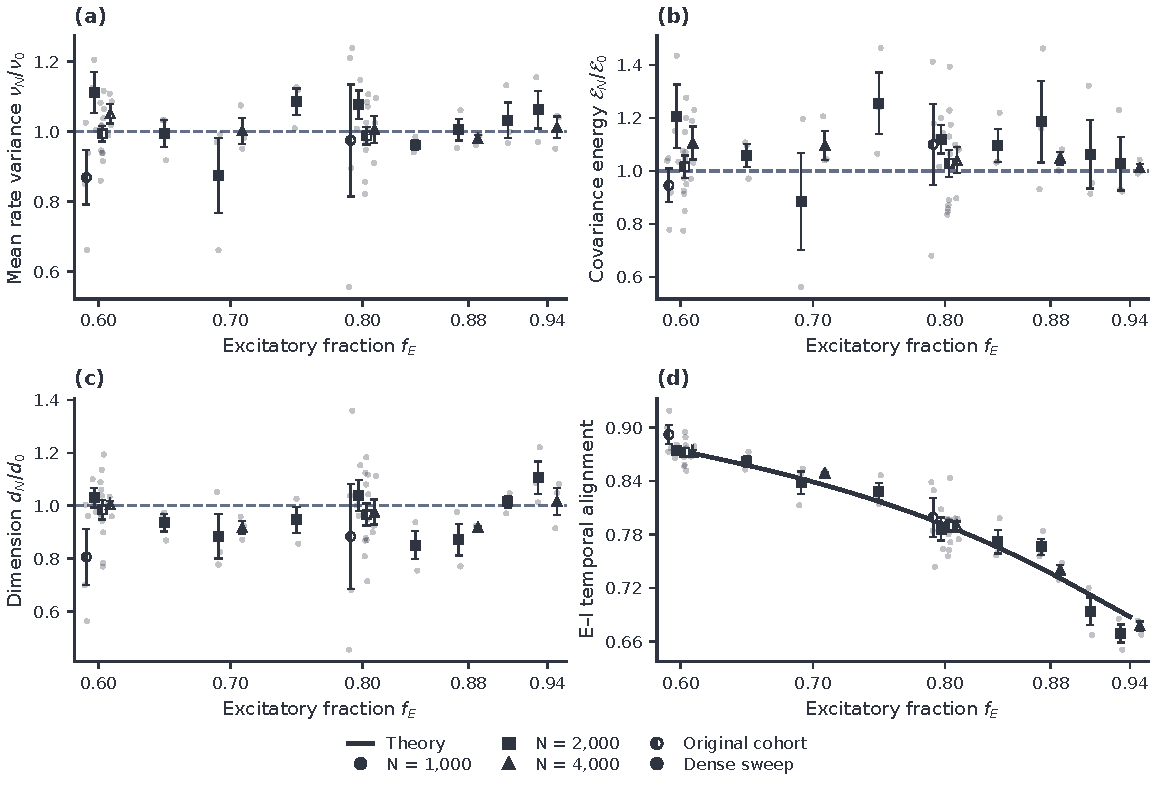
\includegraphics[width=\linewidth]{composition_main.pdf}
\caption{\textbf{Composition changes temporal alignment and the accuracy of the predicted moments.}
The excitatory fraction varies at fixed $J^{0}F$, $GF$, target rates and $\chi=1$.
(a--c) The mean rate variance, covariance energy and joint dimension are divided
by their conditional predictions at each fraction. Dashed lines mark one.
(d) The solid line predicts temporal Gram alignment,
$\mathcal O_{EI}=\energy_{EI}/\sqrt{\energy_{EE}\energy_{II}}$.
Half-filled symbols summarize the original 40 networks at 60:40 and 80:20 E:I.
Filled symbols summarize 36 new networks spanning nine fractions at $N=2000$
and three at $N=4000$, with three connectivity draws at each size and fraction.
Points and bars show individual draws and means with one across-network
standard error. Symbols at the same fraction are offset horizontally.}
\label{fig:composition}
\end{figure}

The composition follow-up sampled $f_E=0.60,0.65,0.70,0.75,0.80,0.84,0.88,
0.91,0.94$ at $N=2000$ and $f_E=0.70,0.88,0.94$ at $N=4000$.
Each setting had three new connectivity seed labels, reused across fractions
for paired comparisons. To compare within-population covariance per available
pair across fractions, we exclude self-pairs and normalize by the number of
distinct ordered pairs.
\begin{equation*}
 P_{aa}=\frac{N}{N_a(N_a-1)}\sum_{\substack{i,j\in a\\i\ne j}} C_{ij}(0)^2,
 \qquad \frac{D_E}{N}=f_E\frac{D_E}{N_E}.
\end{equation*}
The second quantity counts E dimensions at a fixed total network size. For the
fixed aggregate couplings, the theory predicts a maximum of $D_E/N$ at $f_E=0.887$ and minima of the distinct-pair
energies $P_{EE}$ at $0.882$ and $P_{II}$ at $0.768$
(Fig.~\ref{fig:population_sweep}). From $f_E=0.80$ to $0.88$ at $N=2000$,
the paired mean changes in $P_{EE}$ and $P_{II}$ were $+0.002$ (95\% interval
$[-0.325,+0.329]$) and $+0.236$ (95\% interval $[-0.386,+0.858]$).
Both intervals include zero, so these measurements leave the proposed E--E
decrease and I--I increase unresolved.
For $D_E/N$, the pointwise 95\% intervals on the paired changes were
$[-1.97,+1.23]$ percentage points between 0.80 and 0.88 and $[-0.96,+2.16]$ percentage points between 0.88 and 0.94.
The corresponding 0.88-to-0.94 interval at $N=4000$ was $[-0.57,+0.93]$ percentage points.
Each interval uses three matched seed differences. The sampled changes leave the location of an empirical maximum unresolved.

\begin{figure}[t]
\centering
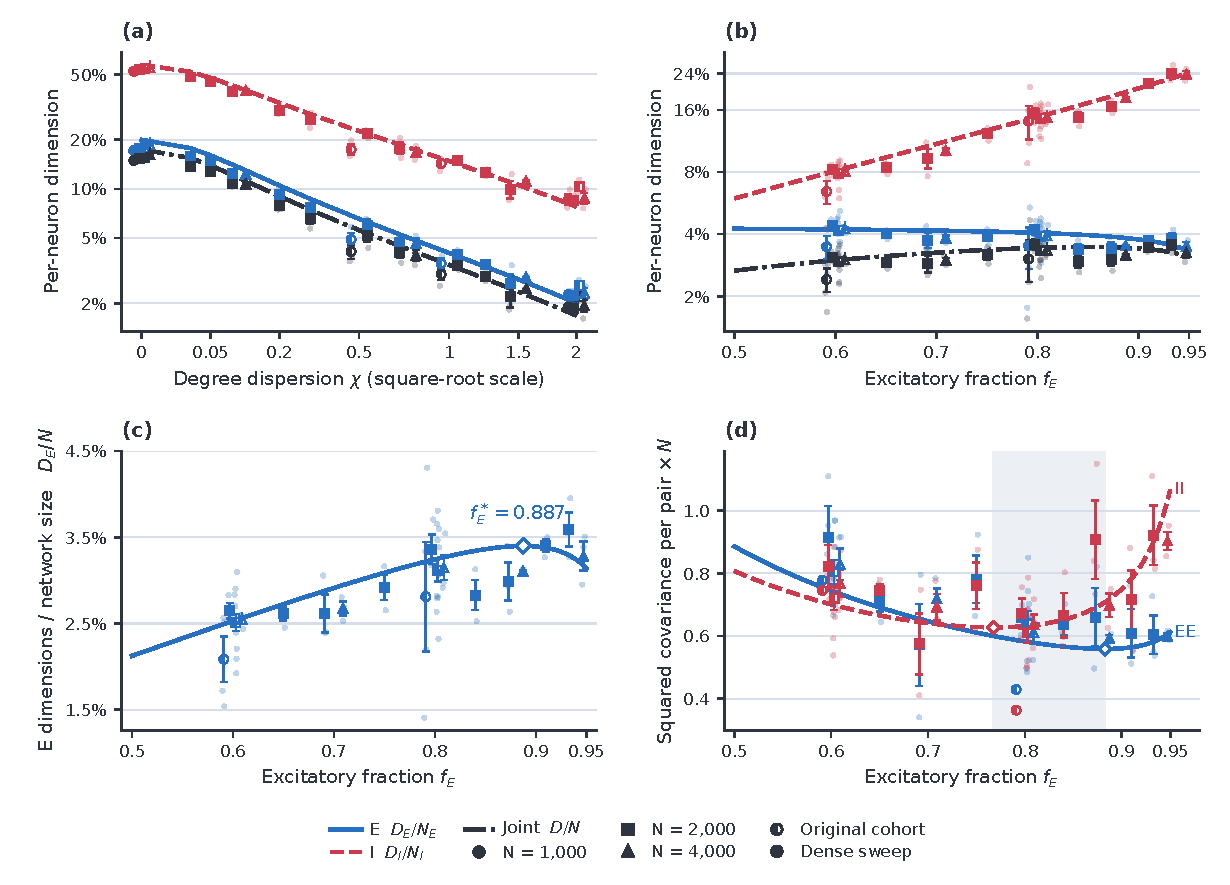
\includegraphics[width=\linewidth]{../figures/population_pr.pdf}
\caption{\textbf{Composition separates per-neuron dimension from total E dimension.}
(a) E-only, I-only and joint participation ratios per corresponding
neuron as degree dispersion changes at 80:20 E:I (square-root horizontal scale).
(b) The same dimensions against excitatory fraction at fixed aggregate couplings
and $\chi=1$. (c) E dimension per network neuron, $D_E/N$. (d) $P_{aa}$,
the mean squared covariance over distinct ordered pairs in population $a$ multiplied
by $N$. Hollow diamonds mark the theoretical extrema. In the shaded interval,
the theory predicts falling $P_{EE}$ and rising $P_{II}$. Faint dots show
networks. Means and one standard error are computed within a cohort, size and
setting. The 69 degree networks enter (a), and all 76 composition networks
enter (b,c). Matched diagonal and block energies are available for 64 of the
composition networks in (d).}
\label{fig:population_sweep}
\end{figure}

The two averaging controls distinguish what these observables test. At
80:20, averaging the gains predicts $\mathcal O_{EI}=0.35138$ instead of
$0.79054$. Averaging the source spectra retains nearly the same alignment,
$0.78766$, but predicts $d=0.07645$ instead of $0.03433$. At $N=2000$, the
measured mean in the original cohort is $0.03316$. Thus alignment alone is insensitive to an
important source-moment approximation, while joint dimensionality and
alignment constrain both response and source heterogeneity. These remain
approximations to the fixed local law, not retuned homogeneous networks.

Population PR illustrates the need to distinguish neuron counts from
absolute dimension. In the original cohort at 80:20 and $N=2000$, the measured per-neuron fractions
are $D_E/N_E=0.03898$ and $D_I/N_I=0.14525$, while their absolute dimensions
are $62.38$ and $58.10$. At 60:40 the absolute values are $50.24$ and
$63.12$. Population dimensions therefore do not simply add to obtain the
whole-network dimension; Eq.~\eqref{eq:jointgeometry} supplies the missing
variance weights and temporal overlap.
Table~\ref{tab:population_dimensions} reports per-neuron and absolute
population dimensions separately.

An ingredient residual remains: the mean squared time-averaged gains at
$N=2000$ lie about $6$--$8\%$ below their predictions. Diagnostic
substitution of measured individual means and temporal variances predicts
the measured gain moment to within about $1\%$ on nine instrumented
networks per composition, while a population Gaussian approximation using
measured $(h,\Delta,q)$ overestimates it by roughly $5$--$8\%$.
Cross-block gain-product checks change the estimate by less than $0.1\%$.
The intermediate substitution of empirical operating points with a common
temporal variance leaves errors of roughly $1.6$--$4.4\%$. Thus both
substitutions reduce the residual in this prescribed diagnostic order.
This locates the dominant tested gain residual in the operating-point
distribution and common-variance approximation, rather than the numerical
gain estimator. It tests the conditional Gaussian one-time marginal mapping,
not the full Gaussian trajectory law. Such same-record calibrated checks are
kept separate from the parameter-only prediction. The good agreement in trace moments and relative
geometry does not establish uniform accuracy of all one-site statistics or
control of the formal finite-size expansion.
At $N=4000$, measured gain moments remain roughly $4$--$7\%$ below
prediction, whereas the empirical individual-moment
calibration errors remain below $0.6\%$ in magnitude. The corresponding
population-Gaussian calibration errors are $3.1$--$5.7\%$
(Table~\ref{tab:gain_calibration}).

Selected step refinements and tangent checks are given in
Appendix~\ref{app:integration_checks}. Four selected PR changes are below
$1.1\%$, but one 80:20, $N=1000$ realization changes by $24.3\%$ and
remains a material sensitivity. A same-step backend change shifts its
8000-time PR by $17.7\%$, and three refined native 16000-time runs still
span $12.3\%$. The tests do not uniquely attribute the discrepancy to
step truncation or establish a converged invariant covariance for this
outlier. The primary outcome is retained. Numerical error therefore cannot be declared uniformly
negligible from these selected checks or from agreement of a PR ratio alone.

The original factor-two 60:40 mismatch does not persist in the tested
larger-network ensemble mean PR. The $N=1000$ deficit remains a
finite-network prediction limitation, with unresolved individual-network
recording and numerical sensitivity; the formal first correction does not
repair it. The
supported resolution is an empirical regime for the ensemble geometry
prediction with a checked recording protocol, rather than a universal
finite-$N$ correction or exact prediction of each circuit.

\subsection{Static and temporal variance must be tested separately}

A finite network can place more input variance in fixed differences between
neurons and less in temporal fluctuations. Testing only the total input
variance $V_a=\Delta_a+q_a$ would miss this change. Let
$\mathcal M_2(h,V,k)=\E[\phi(X_1)\phi(X_2)]$ for two Gaussian variables
with common mean $h$, marginal variance $V$, and covariance $k$. The
conditional Gaussian construction gives
\begin{equation}
 \bar v_a=\mathcal M_2(h_a,V_a,V_a)
          -\mathcal M_2(h_a,V_a,\Delta_a),\qquad
 \left.\frac{\partial\bar v_a}{\partial\Delta_a}\right|_{V_a,h_a}
 =-A_a.
 \label{eq:partitionderivative}
\end{equation}
The second identity follows from Gaussian integration by parts: differentiating
the shared covariance gives $\E[\phi'(X_1)\phi'(X_2)]$, which equals
$\E_z\alpha_a(z)^2=A_a$ at shared covariance $\Delta_a$.
Thus reallocating input variance toward static disorder lowers the temporal
rate variance along this specified diagnostic direction.

At fixed $V,h$, linearizing the static self-consistency functional gives the
susceptibility $(I-W\diag(A))^{-1}$. Its Perron-mode amplification is about
$6.94$ for the reference law. This sensitivity explains why modest changes
in local operating points can matter appreciably for activity fluctuations.
Actual networks also change $V$ and $h$, and the covariance energy changes
through both its source and its response. These derivative identities
therefore diagnose a possible finite-network mechanism; they do not supply
a complete correction to PR.

